\documentclass{standalone}
\usepackage{tikz} 
\usetikzlibrary{shapes.geometric}
 
\begin{document}	
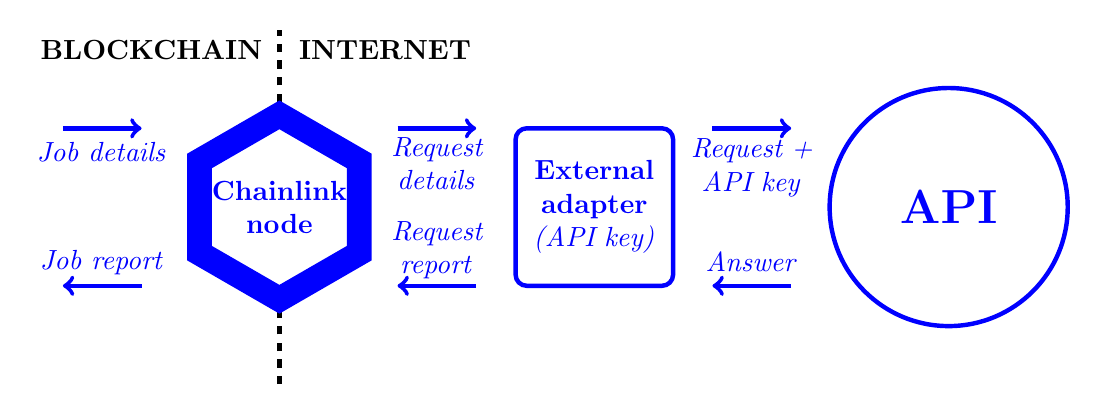
\begin{tikzpicture}

\draw[ultra thick, dashed] (0,-2.25) -- (0,2.25);
\node at (-0.3,2) {\bfseries BLOCKCHAIN \hspace{0.2cm} INTERNET};


\node[rotate=30, draw, regular polygon, regular polygon sides=6, blue, line width=9pt, text width=1.2cm, fill=white] (h2) at (0, 0) {};
\node[blue, text width=2cm, align=center] at (0, 0) {\bfseries Chainlink node};

\node[inner sep=0pt, draw, blue, ultra thick, rounded corners, text width=2cm, align=center, text=blue, minimum height=2cm, text centered] (api) at (4,0) {\textbf{External adapter} \textit{(API key)}};


\node[inner sep=0pt, circle, draw, blue, ultra thick, rounded corners, text width=3cm, align=center, text=blue] (api) at (8.5,0) {\bfseries \LARGE API};


\draw[blue,->,ultra thick] (-2.75,1) -- (-1.75,1);
\node[blue] at (-2.25,0.7) {\textit{Job details}};

\draw[blue,->,ultra thick] (-1.75,-1) -- (-2.75,-1);
\node[blue] at (-2.25,-0.7) {\textit{Job report}};

\draw[blue,->,ultra thick] (1.5,1) -- (2.5,1);
\node[blue, text width=1.5cm, align=center] at (2,0.55) {\textit{Request details}};

\draw[blue,->,ultra thick] (2.5,-1) -- (1.5,-1);
\node[blue, text width=1.5cm, align=center] at (2,-0.55) {\textit{Request report}};

\draw[blue,->,ultra thick] (5.5,1) -- (6.5,1);
\node[blue, text width=1.6cm, align=center] at (6,0.5) {\textit{Request + API key}};

\draw[blue,->,ultra thick] (6.5,-1) -- (5.5,-1);
\node[blue, text width=1.6cm, align=center] at (6,-0.7) {\textit{Answer}};

\end{tikzpicture}
\end{document}